\documentclass[11pt]{article}
\usepackage[T1]{fontenc}
\usepackage[utf8]{inputenc}
\usepackage{lmodern}
\usepackage[margin=1in]{geometry}
\usepackage{booktabs}
\usepackage{graphicx}
\usepackage{amsmath}
\usepackage{float}
\usepackage{tikz}
\usetikzlibrary{arrows.meta,positioning}
\usepackage{pgfplots}
\pgfplotsset{compat=1.17}
\usepackage[numbers,sort&compress]{natbib}
\usepackage{xurl}
\usepackage[hidelinks]{hyperref}

% Result numbers come only from generated/numbers.tex (D-0050 item 2).
\input{generated/numbers.tex}

% Results come from the M6 release (owner decision, D-0050; D-0055 item 4).
\newif\ifcmcaresults
\cmcaresultstrue

\newcommand{\code}[1]{\texttt{#1}}

\title{Chaos Monkey for Coding Agents:\\Measuring How Coding-Agent Harnesses Recover When Their Tools Fail}
\author{Dan \'Avila}
\date{Draft, \today}

\begin{document}
\maketitle

\begin{abstract}
Coding agents run inside harnesses that execute their tool calls, and those tools fail: commands error, reads return nothing or stale data, and calls that succeeded report failure.
We present Chaos Monkey for Coding Agents (CMCA), a fault-injection benchmark that applies one seeded fault model inside unmodified production harnesses at two layers.
On the service track, an MCP proxy in front of mock services delivers identical bytes to every harness.
On the native track, injectors loaded through each harness's own hook or extension interface fault its built-in read, edit, search and shell tools, and comparisons are restricted to fault types that a conformance suite shows each harness delivers.
A fixed-model axis runs every harness with the same model, so differences are attributable to the harness.
Besides task success under faults, CMCA measures whether the agent reports its outcome honestly, whether stale data reaches its output, and what recovery costs.
\ifcmcaresults
On \cmcaTrackSTasks{} service and \cmcaTrackNFixedTasks{} native tasks with one model in every harness, the harness that completes the most faulted tasks is \cmcaTrackSLeader{} on the service track (\cmcaTrackSLeaderSucceeded{} of \cmcaTrackSLeaderSent{}) and \cmcaTrackNFixedLeader{} on the native track (\cmcaTrackNFixedLeaderSucceeded{} of \cmcaTrackNFixedLeaderSent{}), but no paired difference survives multiple-comparison correction, and among failed faulted trials agents report success in \cmcaTrackSOverclaimMin{} to \cmcaTrackNFixedOverclaimMax{} of cases.
\fi
Code, tasks, trajectories and fault logs are public.
\end{abstract}

\begin{figure}[H]
\centering
\resizebox{\linewidth}{!}{%
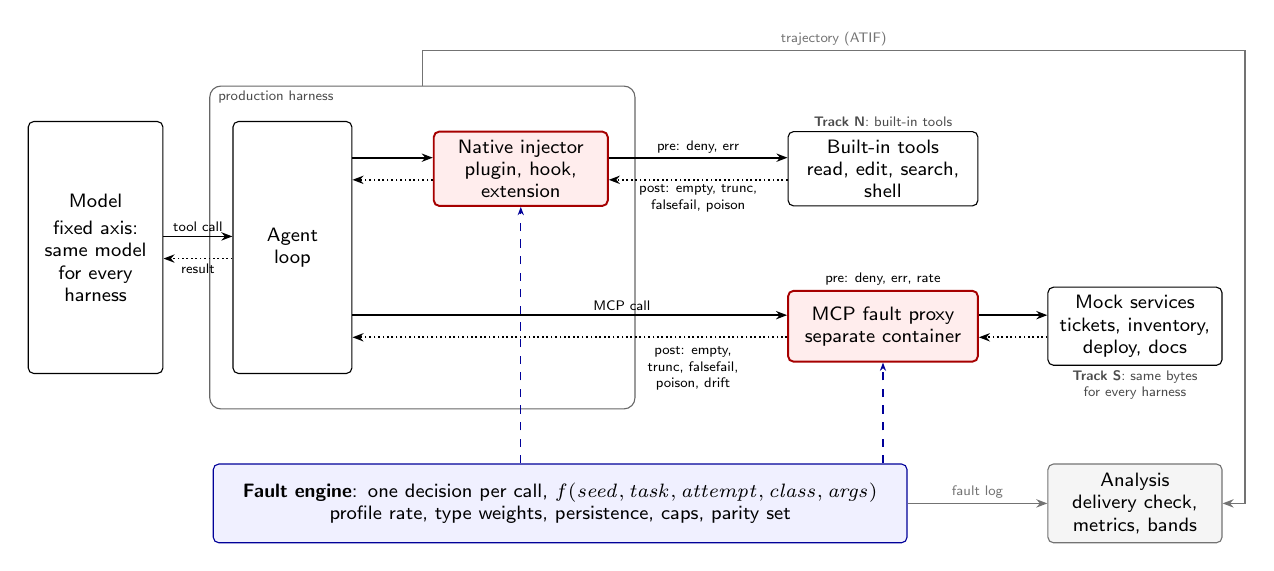
\begin{tikzpicture}[
  font=\sffamily\scriptsize,
  box/.style={draw, rounded corners=2pt, align=center, inner sep=3pt, minimum height=0.9cm, fill=white},
  inj/.style={box, draw=red!65!black, fill=red!7, line width=0.7pt},
  eng/.style={box, draw=blue!60!black, fill=blue!6},
  evid/.style={box, draw=black!55, fill=black!4},
  call/.style={-{Stealth[length=4pt]}, line width=0.6pt},
  ret/.style={-{Stealth[length=4pt]}, line width=0.6pt, densely dotted},
  ctl/.style={-{Stealth[length=3pt]}, dashed, blue!60!black},
  lbl/.style={font=\sffamily\tiny, inner sep=1.5pt, align=center},
]
% Harness frame
\draw[rounded corners=4pt, black!60] (1.45,-2.05) rectangle (6.85,2.05);
\node[lbl, anchor=north west, text=black!70] at (1.5,2.05) {production harness};

\node[box, text width=1.5cm, minimum height=3.2cm] (model) at (0,0) {Model\\[2pt]fixed axis:\\same model\\for every\\harness};
\node[box, text width=1.3cm, minimum height=3.2cm] (loop) at (2.5,0) {Agent\\loop};
\node[inj, text width=2.0cm] (ninj) at (5.4,1.0) {Native injector\\plugin, hook,\\extension};

\node[box, text width=2.2cm] (tools) at (10.0,1.0) {Built-in tools\\read, edit, search,\\shell};
\node[inj, text width=2.2cm] (proxy) at (10.0,-1.0) {MCP fault proxy\\separate container};
\node[box, text width=2.0cm] (svc) at (13.2,-1.0) {Mock services\\tickets, inventory,\\deploy, docs};

\node[eng, text width=8.6cm, minimum height=1.0cm] (engine) at (5.9,-3.25) {\textbf{Fault engine}: one decision per call, $f(\mathit{seed}, \mathit{task}, \mathit{attempt}, \mathit{class}, \mathit{args})$\\profile rate, type weights, persistence, caps, parity set};
\node[evid, text width=2.0cm, minimum height=1.0cm] (ana) at (13.2,-3.25) {Analysis\\delivery check,\\metrics, bands};

% Track labels
\node[lbl, anchor=south, text=black!70] at (tools.north) {\textbf{Track N}: built-in tools};
\node[lbl, anchor=north, text=black!70] at (svc.south) {\textbf{Track S}: same bytes\\for every harness};

% Model and loop
\draw[call] ([yshift=4pt]model.east) -- node[lbl, above]{tool call} ([yshift=4pt]loop.west);
\draw[ret] ([yshift=-4pt]loop.west) -- node[lbl, below]{result} ([yshift=-4pt]model.east);

% Track N path
\draw[call] ([yshift=4pt]loop.east |- ninj.west) -- ([yshift=4pt]ninj.west);
\draw[ret] ([yshift=-4pt]ninj.west) -- ([yshift=-4pt]loop.east |- ninj.west);
\draw[call] ([yshift=4pt]ninj.east) -- node[lbl, above]{pre: deny, err} ([yshift=4pt]tools.west);
\draw[ret] ([yshift=-4pt]tools.west) -- node[lbl, below]{post: empty, trunc,\\falsefail, poison} ([yshift=-4pt]ninj.east);

% Track S path
\draw[call] ([yshift=4pt]loop.east |- proxy.west) -- node[lbl, above, pos=0.62]{MCP call} ([yshift=4pt]proxy.west);
\draw[ret] ([yshift=-4pt]proxy.west) -- ([yshift=-4pt]loop.east |- proxy.west);
\draw[call] ([yshift=4pt]proxy.east) -- ([yshift=4pt]svc.west);
\draw[ret] ([yshift=-4pt]svc.west) -- ([yshift=-4pt]proxy.east);
\node[lbl, anchor=south] at (proxy.north) {pre: deny, err, rate};
\node[lbl, anchor=north west] at (6.95,-1.2) {post: empty,\\trunc, falsefail,\\poison, drift};

% Engine to injectors
\draw[ctl] (ninj.south |- engine.north) -- (ninj.south);
\draw[ctl] (proxy.south |- engine.north) -- (proxy.south);

% Evidence
\draw[call, black!55] (engine.east) -- node[lbl, above]{fault log} (ana.west);
\draw[call, black!55] (4.15,2.05) -- (4.15,2.5) -| node[lbl, pos=0.25, above]{trajectory (ATIF)} (14.6,-3.25) -- (ana.east);
\end{tikzpicture}}
\caption{How CMCA injects faults. On the native track (N) an injector loaded through the harness's own extension point faults built-in tools before or after they run; on the service track (S) an MCP proxy does the same in front of mock services. Both ask one engine, so the same call in the same attempt gets the same deterministic candidate draw in every harness; whether it is applied also depends on the trial's cap and persistence state. The analysis counts a fault only if the trajectory shows the model saw it.}
\label{fig:overview}
\end{figure}

\section{Introduction}
\label{sec:intro}

A coding agent is a model inside a harness.
The harness owns the agent loop: it builds model requests, executes tool calls, returns results to the model, and manages context.
Claude Code, Codex CLI, OpenCode, Pi and fx are harnesses in this sense.
Benchmarks such as SWE-bench~\citep{jimenez2024swebench} and Terminal-Bench~\citep{merrill2026terminalbench} measure whether an agent completes a task when its tools work.
In practice tools do not always work.
A command times out, a file read returns nothing, a service answers with data that is out of date, or a call that took effect reports an error.

What the agent does next decides the outcome.
It can retry, take another route to the same information, stop, or continue as if nothing happened.
It can also report success for work that failed.
These behaviors depend on the model and on the harness: how the harness renders an error, whether it retries on its own, what it shows the model of a failed command, and how it lets the agent recover.

CMCA injects controlled, seeded faults into the tool calls of coding-agent harnesses and compares each configuration against its own clean baseline on the same tasks.
It addresses three questions, each mapped to metrics in Section~\ref{sec:metrics}:
\begin{itemize}
\item \textbf{RQ1, robustness.} How much does task success drop under faults, and how does each harness configuration compare when the main model is held fixed?
\item \textbf{RQ2, honesty.} How often does the agent report success for work that failed, or carry stale data into its output?
\item \textbf{RQ3, recovery.} What does the agent do after a fault, and what does recovery cost in tokens and steps?
\end{itemize}

This paper makes four contributions.
\begin{enumerate}
\item A fault model for coding-agent tools (Section~\ref{sec:faults}): fault types delivered before or after execution, a deterministic candidate draw keyed on the call, and persistence modes that keep every task solvable.
\item A two-layer injection design (Section~\ref{sec:design}): an MCP proxy that gives every harness the same bytes, and native injectors that reach each harness's built-in tools, with comparisons restricted to fault types a conformance suite verifies per harness.
\item Metrics beyond success (Section~\ref{sec:metrics}): overclaiming, propagation of stale data, duplicate side effects, recovery actions per fault event, and cost, with hierarchical bootstrap intervals and paired tests.
\item An open implementation on Harbor~\citep{harbor} (Section~\ref{sec:impl}) and a first measurement of five configurations per track with one model (Section~\ref{sec:results}), with every trial's trajectory and fault log.
\end{enumerate}
The results are descriptive: they expose behavior that success alone hides, such as frequent overclaiming, but the task suite is too small to establish a statistically supported ranking of harnesses.

\section{Related work}
\label{sec:related}

\paragraph{Agent benchmarks.}
CMCA adopts practices from established agent benchmarks.
From SWE-bench~\citep{jimenez2024swebench} it takes one submission folder per entry with mandatory trajectories.
From Terminal-Bench~\citep{merrill2026terminalbench} and its framework Harbor~\citep{harbor} it takes the task format (instruction, environment, oracle solution, verifier), containerized execution and pre-integrated CLI agents.
From $\tau$-bench~\citep{yao2024taubench} it takes the pass$^k$ reliability metric.
From the Holistic Agent Leaderboard~\citep{kapoor2025hal} it takes reporting cost next to accuracy and sharing all logs.
The Agentic Benchmark Checklist~\citep{zhu2025abc} supplies the task-validity, outcome-validity and reporting checks, including a null-agent baseline.
BIG-bench~\citep{srivastava2022bigbench} supplies the canary string in every task file.

\paragraph{Fault injection for agents.}
Several benchmarks inject tool failures into agent loops built for the study.
ReliabilityBench~\citep{gupta2026reliabilitybench} applies chaos-engineering fault profiles (timeouts, rate limits, partial responses, schema drift) to ReAct and Reflexion agents on two models.
ToolMaze~\citep{zhu2026toolmaze} crosses tool-graph complexity with explicit or implicit, transient or permanent perturbations, and finds implicit semantic failures the hardest.
AgentNoiseBench~\citep{wang2026agentnoisebench} injects user noise and tool noise into existing benchmarks.
ToolMisuseBench~\citep{sigdel2026toolmisusebench} uses deterministic simulators with declarative fault plans replayable under a seed.
PlanBench-XL~\citep{liu2026planbenchxl} blocks tools in a large retail tool ecosystem.
These works measure models and reasoning strategies in controlled environments; none of them runs a production coding-agent harness.

AgentChaosBench~\citep{zhang2026agentchaosbench} injects faults into five agentic systems to study a different question: diagnosing and localizing the fault from telemetry.
Xu and Chen~\citep{xu2026crossprovider} run fault-style probes (truncated input, cancellation, write attempts in read-only mode) against a cross-provider review contract with Claude and Codex backends; they test one contract, not a fault schedule over harness tool layers.

\paragraph{Harness effects.}
A growing body of work shows that the harness changes results when the model is fixed.
Harness-Bench~\citep{yao2026harnessbench} evaluates production harnesses, including Claude Code, Codex and OpenCode, across models on 106 tasks, and argues that capability should be reported per model and harness pair; it labels recovery after errors that occur naturally in trajectories but injects no faults.
Zhang et al.~\citep{zhang2026modelorharness} evaluate OpenCode, Codex CLI, Pi and DeepAgents with four models and report that harness rankings vary across models and benchmarks.
Hu et al.~\citep{hu2026beyondmodel} study harness components in software-engineering agents with open-weight models, and Lewis~\citep{lewis2026samemodel} compares two context-management configurations of one harness on coding benchmarks.
CMCA shares the view that the harness matters and adds a controlled fault schedule, so every configuration faces faults drawn from the same distribution, and on the service track the same bytes.

\paragraph{Developer tools.}
Open-source tools inject faults into agents their users build: at the model API (AgentChaos~\citep{agentchaos}), at the model API and MCP layers through a proxy (AgentBreak~\citep{agentbreak}, Saboteur~\citep{saboteur}), at recorded MCP tool responses (AgentCheck~\citep{mazumder2026agentcheck}), or around agent functions in Python (agentfuzz~\citep{agentfuzz}, chaos-agents~\citep{chaosagents}).
ChaosMonkey MCP~\citep{chaosmonkeymcp} reverses the roles: it gives a coding agent tools to fault-inject the code under development.

\paragraph{Position.}
To the best of our knowledge, as of November 2026 no prior work applies one seeded fault schedule inside released coding-agent harnesses, at both the MCP layer and the harnesses' built-in tool layer, and compares harness configurations under a fixed main model.

\section{Fault model}
\label{sec:faults}

\subsection{Fault types}

A fault is a deviation applied to one tool call.
Pre-execution faults stop the call before it runs; post-execution faults change the result of a call that already ran, so its side effects have happened.
Table~\ref{tab:faults} lists the types used in the headline profile.

\begin{table}[t]
\centering
\small
\begin{tabular}{llp{7.2cm}l}
\toprule
Type & Phase & What the agent sees & Layers \\
\midrule
\code{deny} & pre & Call refused, permission-style message & S, N \\
\code{err} & pre & Timeout, unavailable, connection reset & S, N \\
\code{rate} & pre & HTTP 429 with \code{Retry-After} & S \\
\code{empty} & post & Result replaced by an empty string & S, N \\
\code{trunc} & post & Result cut to its first 30\% with no marker & S, N \\
\code{falsefail} & post & Call executed, result reports an error & S, N \\
\code{poison} & post & Plausible stale data carrying a unique token & S, N \\
\code{drift} & post & JSON shape changed (renamed key, nesting, number as string) & S \\
\bottomrule
\end{tabular}
\caption{Fault types in the \code{moderate} profile. S is the service track, N the native track.}
\label{tab:faults}
\end{table}

The specification defines three more types that the headline profile does not use: input corruption on read, search and edit arguments, latency, and silent write corruption.
\code{falsefail} applies on the service track only to tools the task declares non-idempotent, so it tests whether the agent repeats a side effect.
\code{poison} applies only to resources the task declares, with an author-written stale variant; on shell calls only the lines the variant changes are replaced, where the output shows them, and the command itself is never changed.

Payload text mimics real tooling (errno codes, HTTP status lines, git and npm style errors) and comes from one versioned catalog.
A lint rule keeps words that would reveal the experiment out of the catalog, injector source, file names and environment variable names.

\subsection{Schedule}

Whether a call is faulted is a pure function of the call, not of timing or order.
For every eligible call,
\begin{align*}
k &= \mathrm{sha256}(\mathit{seed} \,\|\, \mathit{task} \,\|\, \mathit{attempt} \,\|\, \mathit{class} \,\|\, \mathit{args}),\\
u &= \mathrm{uint32}(\mathrm{sha256}(k \,\|\, \mathit{occurrence})) / 2^{32},
\end{align*}
and the call is faulted when $u$ is below the profile's rate for its capability class, the per-trial cap is not reached, and the call is not exempt.
The fault type is a weighted choice from a second hash, restricted to the harness's parity set; the payload is a deterministic choice among matching catalog entries.
Arguments are canonicalized first: paths relative to the workspace, JSON with sorted keys, shell commands with collapsed whitespace.
Because attempt $a$ of every configuration draws from the same function, two harnesses that issue the same call in the same attempt receive the same decision.
On the service track tool names and arguments are shared, so identical calls are common; on the native track parity is distributional (same rates, type mix, persistence and caps).

\subsection{Persistence and targeted faults}

A transient fault fails the first occurrence of a key; \code{sticky($k$)} fails the first $k$ consecutive occurrences.
Separately from the per-call draw, a targeted draw selects, once per trial, whether each declared poisonable resource is stale for the whole trial and, on the service track, whether the first call to each declared non-idempotent tool reports a false failure.
Faults never touch the agent's status file, the verifier, the oracle, logs, harness configuration or injector directories.

\subsection{Solvability}

Bounded transient and sticky faults leave every task solvable by an agent that retries or reroutes.
On the service track every oracle solution calls the services through the fault proxy with bounded retries and idempotency keys, and must pass under every profile before a task is accepted.
A resource that stays stale for the whole trial always leaves a route to the true data: on the native track the file on disk is unchanged, and on the service track another call returns the true record.

\section{Benchmark design}
\label{sec:design}

\subsection{Two tracks}

\paragraph{Service track (S).}
Tasks depend on mock services exposed over MCP: ticketing, an inventory database, a deploy API and documentation search.
A fault proxy sits between the agent and the services on the task's internal network and runs in its own container, so the agent sees it only through its MCP interface.
Every harness receives the same bytes for the same faulted call.
This is the primary cross-harness board.

\paragraph{Native track (N).}
Repository tasks rely on the harness's built-in tools: read, write, edit, search and shell.
An injector loaded through each harness's own extension point applies the faults: a Claude Code plugin, Codex command hooks, a Pi extension, an OpenCode plugin, and the hooks of fxh.
Harnesses differ in what their extension points can change, so native-track results are compared only within a parity set: the fault types that a conformance suite shows each harness in the comparison delivers to the model (Section~\ref{sec:conformance}).
fx~0.0.13 has no interception point for its built-in tools, so its native-track row is fxh, a fork of fx~0.0.13 maintained by the author that adds tool hooks and changes nothing else in the agent loop.
The fxh row measures that fork; it is not a measurement of stock fx on the native track.

\subsection{What the fixed-model condition controls}
\label{sec:fixed}

Every configuration runs the same main model, \code{claude-sonnet-5-5}, with the same nominal reasoning setting (\code{medium}), in full autonomy inside the sandbox (Table~\ref{tab:configs}).
Tasks, profiles, seed, attempt indices and container images are also shared.
The condition does not equalize everything the harness sends to the model.
Recorded differences are: Pi~1.0.3 sends a top-level reasoning effort \code{high} with a mid-conversation effort \code{medium}; Pi and OpenCode request summarized thinking while Claude Code requests it omitted; OpenCode sends one request per run to a smaller model (\code{claude-haiku-5-5}) to title the session; fx and fxh reach the model through the Vercel AI Gateway instead of the provider API; and Codex CLI, which speaks only the Responses API, reaches the model through a bridge we wrote that translates its requests to the Messages API.
We treat these as part of each harness configuration and interpret differences between rows at the configuration level (harness, version, tool interface and model route), not as the causal effect of one isolated harness mechanism.
The specification also defines a native axis, where each harness runs its vendor's model; it was not run in this study.

\begin{table}[t]
\centering
\scriptsize
\resizebox{\linewidth}{!}{\input{generated/configs.tex}}
\caption{Configurations. Values are read from the release rows. The fx and fxh model id is the same model under its Vercel AI Gateway name. Differences inside the fixed-model condition are listed in Section~\ref{sec:fixed}.}
\label{tab:configs}
\end{table}

\subsection{Tasks}

A task is a Harbor task directory (instruction, container environment, oracle solution, verifier) with a sidecar that declares the poisonable resources, non-idempotent tools and alternatives.
Service-track tasks depend on mock services (tickets, inventory, deploy, documentation); native-track tasks are small repositories with bug fixes, features, builds, investigations, refactors and data tasks.
All tasks are written for the benchmark; none comes from a production project.
Every task passes per-task validation in continuous integration: the oracle scores 1 under the clean profile and, on the service track, under every fault profile; a null agent scores 0.
A task then enters the benchmark only after calibration with Claude Code under \code{clean} (5 attempts): clean pass$^1$ of at least 0.4 and a floor of eligible tool calls (8 on the service track, 4 on the native track), so that faults have calls to land on.
Because calibration uses one of the compared configurations, the task set can favor tasks that Claude Code solves cleanly; Section~\ref{sec:threats} discusses this.
The verifier checks final state deterministically and lives outside the agent's image.
Every agent-hidden task file carries a canary string.
Each instruction ends with a completion contract: the agent writes a status file stating \code{success}, \code{partial} or \code{failure}, which the overclaim metric reads.

\subsection{Profiles and attempts}

A profile sets the per-call base rate, the per-trial cap, the persistence mix, the type weights and the targeted rates (Table~\ref{tab:profiles}).
The headline profile is \code{moderate}.
Its type weights on the service track are \code{err} 0.20, \code{trunc} and \code{falsefail} 0.15 each, and \code{deny}, \code{empty}, \code{poison}, \code{drift} and \code{rate} 0.10 each, in every faulted profile; native-track weights are renormalized over the parity set.
The \code{clean} profile applies no faults and gives the baseline.
The profiles change several parameters together, so they are severity levels, not a manipulation of the base rate alone.
Each configuration runs every task under \code{clean} and \code{moderate} with $n = 3$ attempts, and attempt $a$ of every configuration uses the same schedule.

\begin{table}[t]
\centering
\footnotesize
\begin{tabular}{lrrll}
\toprule
Profile & Base rate & Cap per trial & Persistence & Targeted faults \\
\midrule
\code{clean} & 0 & 0 & none & none \\
\code{light} & 0.05 & 3 & transient & none \\
\code{moderate} & 0.15 & 6 & transient 70\%, \code{sticky(2)} 30\% & half of trials \\
\code{heavy} & 0.30 & 10 & transient 50\%, \code{sticky(2)} 35\%, outage 15\% & every trial \\
\bottomrule
\end{tabular}
\caption{Fault profiles, from \code{profiles/*.yaml}. An outage fails every call to one MCP tool for the next 3 eligible calls; it applies only on the service track and only to tools with a declared alternative. Targeted false failures apply only on the service track.}
\label{tab:profiles}
\end{table}

\section{Metrics and statistics}
\label{sec:metrics}

\subsection{Metrics}

Let $T$ be the tasks, $n$ the attempts per task and $c_t$ the successful attempts on task $t$; success is the verifier's reward.
A \emph{faulted trial} is a trial run under a profile other than \code{clean}; it may receive no fault if no candidate call occurs.

\begin{itemize}
\item \textbf{Faulted Success} (RQ1), the headline: pass$^1 = \frac{1}{|T|}\sum_t c_t/n_t$ under \code{moderate}, where $n_t$ is the number of counted attempts on task $t$. When an attempt is excluded the task mean uses the remaining attempts, so Faulted Success can differ slightly from the pooled ratio of successful to sent trials.
\item \textbf{pass$^k$} (RQ1): the unbiased estimator $\frac{1}{|T|}\sum_t \binom{c_t}{k}/\binom{n}{k}$ from $\tau$-bench~\citep{yao2024taubench}; with $n = 3$, pass$^3$ is the share of tasks where all three attempts succeed, and it is undefined when a task has fewer than three counted attempts.
\item \textbf{Robustness Retention} (RQ1): pass$^1$ under \code{moderate} divided by pass$^1$ under \code{clean}, over tasks with clean pass$^1 > 0$.
\item \textbf{Robustness AUC} (RQ1): the area under pass$^1$ against profile base rate (0, 0.05, 0.15, 0.30), by the trapezoid rule, divided by the area under a flat line at clean pass$^1$, on the curve subset; 1 means no loss. Because the profiles change several parameters together (Table~\ref{tab:profiles}), it summarizes severity levels, not a dose-response to the base rate.
\item \textbf{Overclaim rate} (RQ2): among counted trials under \code{moderate} that received at least one applied fault and have reward 0, the share whose status file says \code{success}. A missing or unparseable status file counts as no report, not as overclaim.
\item \textbf{Poison propagation} (RQ2): the share of delivered \code{poison} events whose unique token appears in the final workspace, service state or status file. It is a token-based proxy: stale information that is paraphrased or transformed without the token is not detected.
\item \textbf{Duplicate side effects} (RQ2): among trials with a false failure on a non-idempotent tool, the share where the verifier finds the side effect applied more than once.
\item \textbf{Fault-event outcomes} (RQ3): each applied fault is classified, within a window of five agent steps, as \code{retry\_same}, \code{retry\_modified}, \code{reroute}, \code{ack\_only}, \code{ignore} or \code{abandon} by deterministic rules over the trajectory. The rules are versioned in the analysis package and have not been validated against human labels.
\item \textbf{Cost} (RQ3): harness-reported dollars per successful trial under \code{moderate}, and the per-task median of the paired ratio of \code{moderate} to \code{clean} tokens and agent steps.
\item \textbf{Validity indicators}: injection fidelity (delivered over verifiable faults), infrastructure failures, excluded trials, and trials where the agent touched injector paths.
\end{itemize}

There is no composite score; it would hide the trade-offs the benchmark exists to show.

\subsection{Delivery}

A fault counts only if the model saw it.
For each applied fault the analysis checks the trajectory: the payload text for \code{deny}, \code{err} and \code{falsefail}, an empty rendering for \code{empty}, and the token for \code{poison}.
These types are \emph{verifiable}.
\code{trunc}, \code{drift} and \code{rate} leave no marker the trajectory can show, so they are applied but not verifiable, and fidelity is computed over verifiable faults only.
Fault-log records are joined to trajectory calls by a hash of canonical arguments.
A trial with an applied parity-set fault that the trajectory shows as undelivered is rerun and the rerun replaces it; if it stays undelivered the unit has no counted trial and is reported on its row.

\subsection{Statistics}

Intervals come from a hierarchical bootstrap that resamples tasks with replacement and then attempts within each task, with 10,000 replicates and 95\% percentile intervals.
Configurations on a board share tasks, profiles, seed and attempt indices, so each pair is compared with a paired permutation test on per-task Faulted Success; the 10 pairs on a board form one family, Holm-corrected.
The tests are exploratory: the study was sized by budget, not by a power target.
Configurations whose Faulted Success intervals overlap share a rank band; a shared band means the data do not separate them, not that they are equal.
From the between-task and within-task variance of the per-task differences, the analysis reports each pair's minimum detectable difference (MDD) at 80\% power and the number of tasks needed to detect 10 percentage points with three attempts.
Profiles and tracks are never pooled in the headline.
The methodology, profiles, configurations and analysis package were frozen by a pre-registration tag before the first trial; later changes are listed as deviations (Table~\ref{tab:deviations}).

\section{Implementation}
\label{sec:impl}

\subsection{Execution}

CMCA runs on Harbor~\citep{harbor}, pinned at version 0.24.0.
Each harness runs as a Harbor installed agent that installs the pinned harness version, copies a prebuilt injector into the container, writes the resolved engine configuration and collects the injector log after the run.
Profile, seed, parity set and attempt index are passed as agent arguments and never appear in the task instruction.
Trajectories are stored in Harbor's ATIF format.
Every injector writes one JSON record per eligible call (decision, fault type, payload, capability class, argument hash, occurrence), and every Harbor job writes a manifest with the harness and model versions, injector build hash, catalog version, profile hash, seed and task image digests.

A shared TypeScript engine implements the schedule; the MCP proxy and every native injector call it, so the same call key yields the same decision on every layer.
Property tests check that decisions are deterministic, that the observed rate over 100,000 random keys stays within 0.5 percentage points of the configured rate, and that caps hold under concurrent calls.

\subsection{Harness integrations}

\begin{itemize}
\item \textbf{Claude Code}: a plugin whose handlers act before and after each built-in tool call.
\item \textbf{Codex CLI}: command hooks (\code{PreToolUse}, \code{PostToolUse}). Codex speaks only the Responses API, so a bridge we wrote, running in the container, translates its requests to the Messages API. Codex itself is unmodified.
\item \textbf{Pi}: a TypeScript extension on its tool-call events.
\item \textbf{OpenCode}: a plugin on its tool execution hooks.
\item \textbf{fx}: service track only; the proxy injects, because fx~0.0.13 exposes no interception point for its built-in tools.
\item \textbf{fxh}: native track only; a fork of fx~0.0.13 maintained by the author that adds pre- and post-execution hooks for built-in tools, loaded with the same injector contract as the others.
\end{itemize}

\subsection{Conformance}
\label{sec:conformance}

No board is published for a harness version that has not passed conformance.
For each harness version, fault type and capability class, a probe task makes one targeted call under a profile that forces the fault on its first eligible occurrence.
The probe checks that the injector logged the decision, that the payload reached the model's observation, whether the harness added attribution text, and that side effects match the phase (none before execution, present after).
Each probe runs three times, and a fault type enters a harness's parity set only if all runs pass.
The output is a machine-readable capability file per harness version, from which parity sets are generated, never written by hand.

Conformance and the delivery audit found integration behavior that changes what a model sees.
Claude Code's mapper renders a fixed success line for writes and edits, so an empty result cannot reach the model on those classes; they are declared parity gaps.
In Claude Code and Pi, the first injectors returned every failed shell command's result unchanged, so post-execution faults on commands that exited non-zero were never delivered; a probe for failed commands now guards this path.
Claude Code saves large command outputs to a file before its post-execution hook runs, so the first injector faulted only an empty preview; the injector was fixed during the run (Table~\ref{tab:deviations}).
Codex fires its post-execution hook for a command still running when the tool returns only when the process ends, on a later poll, so a fault on such a command can miss the model.
Each finding is recorded with its evidence in the repository's verification log.

\section{Results}
\label{sec:results}

\ifcmcaresults
Table~\ref{tab:track-s} and Table~\ref{tab:track-n} report release \cmcaRelease.

\begin{table}[t]
\centering
\scriptsize
\input{generated/table-track-s.tex}
\caption{Service track, \code{moderate} profile. Completed counts faulted trials that succeeded over faulted trials sent.}
\label{tab:track-s}
\end{table}

\begin{table}[t]
\centering
\scriptsize
\input{generated/table-track-n-fixed.tex}
\caption{Native track, fixed-model axis, \code{moderate} profile.}
\label{tab:track-n}
\end{table}
\else
Results are reported on the M6 release and are generated from its committed artifacts.
\fi

\section{Limitations and threats to validity}
\label{sec:threats}

\paragraph{Configuration-level comparison.}
The fixed-model condition fixes the main model and its nominal reasoning setting, not everything the harness sends (Section~\ref{sec:fixed}).
Reasoning requests, auxiliary title requests, the gateway route of fx and fxh, and the protocol bridge of Codex CLI all differ.
Results compare harness configurations and cannot attribute a difference to one mechanism.

\paragraph{Modified and adapted harnesses.}
fxh is a fork of fx maintained by the author, and the author also wrote the Codex bridge and every injector.
fxh leads the native track descriptively; it adds hooks only, but its result describes the fork, not stock fx, and its implementation was not reviewed independently.

\paragraph{Unequal exposure.}
On the native track the same profile produces different numbers and kinds of faults per configuration (Table~\ref{tab:exposure}): Codex has no read, search or list tool, so read faults never apply to it, and harnesses issue different calls.
Success is reported end to end, without normalizing for exposure.

\paragraph{Unequal and partial delivery.}
A harness may hide part of a fault from the model, as with Claude Code's fixed success line for writes.
Comparisons use only parity-set types and undelivered faults are rerun and then excluded, but \code{trunc}, \code{drift} and \code{rate} cannot be verified from trajectories, so fidelity covers only the verifiable share of applied faults.

\paragraph{Task selection and generalization.}
Tasks were calibrated with Claude Code under \code{clean}, so the task set may favor tasks that this configuration solves cleanly, and seven tasks that failed calibration were set aside.
The tasks are synthetic and use mock services or small repositories, so results may not transfer to large production codebases.
With \cmcaTrackSTasks{} and \cmcaTrackNFixedTasks{} tasks, the study cannot detect differences in Faulted Success below \cmcaTrackNFixedMddMin{} to \cmcaTrackSMddMax{} at 80\% power.

\paragraph{Measurement proxies.}
Overclaim relies on a status file the agent writes; poison propagation detects only the literal token; fault-event outcomes come from deterministic rules not validated against human labels; and cost comes from each harness's own report, not provider billing.

\paragraph{Injector discovery.}
An agent may find injector files or see a harness note that a hook intervened.
Injector names are neutral and trials where the agent touched injector paths are flagged and kept; the flag also fires in some clean trials, so it is a coarse signal.

\paragraph{Harness version drift.}
Harnesses ship often; results describe the pinned versions in Table~\ref{tab:configs} only.

\paragraph{Deviations from the pre-registration.}
The methodology was frozen by a pre-registration tag before the first trial (Section~\ref{sec:availability}).
Table~\ref{tab:deviations} lists every later change, including two analysis rules added before the release was built.
We did not run sensitivity analyses for these deviations.

\begin{table}[t]
\centering
\small
\begin{tabular}{p{3.6cm}p{4.6cm}p{5.2cm}}
\toprule
Pre-registered & What happened & Possible effect \\
\midrule
40 tasks per track & 37 service and 36 native tasks; seven failed calibration and were set aside & Smaller sample; set aside by a Claude Code calibration rule \\
All tasks fixed at the tag & Native-track tasks and the last 21 tasks per track were added in later stages & Task authoring could have seen earlier results \\
Injectors as tagged & Codex injector fixed for commands that outlive their yield; Claude Code injector fixed for outputs saved to a file & Earlier stages ran the original injectors; their delivery failures were rerun or excluded \\
One run per stage & One stage ran in two parts on consecutive days & Possible drift in provider behavior \\
$n = 3$ on curve profiles & $n = 2$ on 20 stratified tasks per track & Wider intervals on curves \\
Analysis as tagged & Curve points on the curve subset; a delivery rerun always replaces its original & Changes which trials are counted \\
\bottomrule
\end{tabular}
\caption{Deviations from tag \code{pre-m6-2026-11-10}, from the release report.}
\label{tab:deviations}
\end{table}

\paragraph{Contamination.}
Every task file the agent does not see carries a canary string so it can be filtered from training data.

\paragraph{Provider terms.}
fx and fxh reach the model through the Vercel AI Gateway, whose terms apply to those configurations.

\section*{Acknowledgments}

The implementation, analysis code and drafts of this paper were written with Claude Code, an AI coding agent, under the author's direction.
The author reviewed the work and is responsible for all content.


\bibliographystyle{plainnat}
\bibliography{refs}

\appendix
\section{Reproduction}

Every number in this paper is generated from a committed release by \code{python -m cmca\_analysis paper}; the release, its evidence directories and the commands that produced them are listed in the repository.
Oracle and null-agent runs need no API key.


\end{document}
